Een Linux server die ge\"installeerd is zonder grafische interface heeft op zijn monitor de prompt Login: daar kan je
inloggen als gebruiker. Via de toets combinatie ALT en F1-F6 kan je schakelen naar verschillende consoles zodat je
meerdere keren ingelogd kan zijn.

Omdat wij werken vanuit een virtual machine is het werken met een console niet makkelijk en gebruiken we een terminal
applicatie. Start Terminal of Terminal Emulator vanaf de Dash, zie figuur \ref{fig:DashTerminal}

\begin{figure}
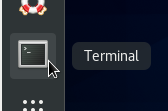
\includegraphics{linuxreader-img021.png}
	\label{fig:DashTerminal}
	\caption{Terminal op de Dash}
\end{figure}

